\chapter{Virittävät puut}

\index{virittxvx puu@virittävä puu}

\key{Virittävä puu} on kokoelma
verkon kaaria,
joka kytkee kaikki
verkon solmut toisiinsa.
Kuten puut yleensäkin,
virittävä puu on yhtenäinen ja syklitön.
Virittävän puun muodostamiseen
on yleensä monia tapoja.

Esimerkiksi verkossa
\begin{center}
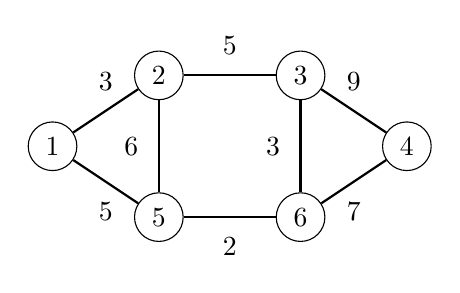
\begin{tikzpicture}[scale=0.9]
\node[draw, circle] (1) at (1.5,2) {$1$};
\node[draw, circle] (2) at (3,3) {$2$};
\node[draw, circle] (3) at (5,3) {$3$};
\node[draw, circle] (4) at (6.5,2) {$4$};
\node[draw, circle] (5) at (3,1) {$5$};
\node[draw, circle] (6) at (5,1) {$6$};
\path[draw,thick,-] (1) -- node[font=\small,label=above:3] {} (2);
\path[draw,thick,-] (2) -- node[font=\small,label=above:5] {} (3);
\path[draw,thick,-] (3) -- node[font=\small,label=above:9] {} (4);
\path[draw,thick,-] (1) -- node[font=\small,label=below:5] {} (5);
\path[draw,thick,-] (5) -- node[font=\small,label=below:2] {} (6);
\path[draw,thick,-] (6) -- node[font=\small,label=below:7] {} (4);
\path[draw,thick,-] (2) -- node[font=\small,label=left:6] {} (5);
\path[draw,thick,-] (3) -- node[font=\small,label=left:3] {} (6);
\end{tikzpicture}
\end{center}
yksi mahdollinen virittävä puu on seuraava:
\begin{center}
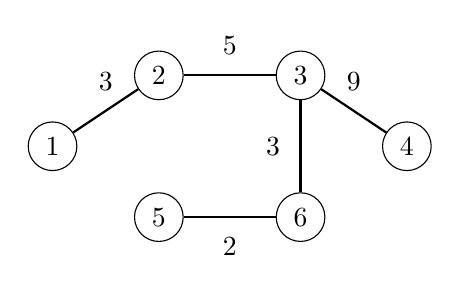
\begin{tikzpicture}[scale=0.9]
\node[draw, circle] (1) at (1.5,2) {$1$};
\node[draw, circle] (2) at (3,3) {$2$};
\node[draw, circle] (3) at (5,3) {$3$};
\node[draw, circle] (4) at (6.5,2) {$4$};
\node[draw, circle] (5) at (3,1) {$5$};
\node[draw, circle] (6) at (5,1) {$6$};
\path[draw,thick,-] (1) -- node[font=\small,label=above:3] {} (2);
\path[draw,thick,-] (2) -- node[font=\small,label=above:5] {} (3);
\path[draw,thick,-] (3) -- node[font=\small,label=above:9] {} (4);
\path[draw,thick,-] (5) -- node[font=\small,label=below:2] {} (6);
\path[draw,thick,-] (3) -- node[font=\small,label=left:3] {} (6);
\end{tikzpicture}
\end{center}

Virittävän puun paino on siihen kuuluvien kaarten painojen summa.
Esimerkiksi yllä olevan puun paino on $3+5+9+3+2=22$.

\key{Pienin virittävä puu}
on virittävä puu, jonka paino on mahdollisimman pieni.
Yllä olevan verkon pienin virittävä puu
on painoltaan 20, ja sen voi muodostaa seuraavasti:

\begin{center}
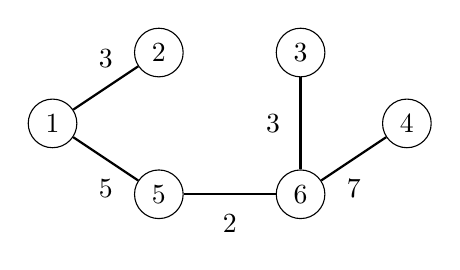
\begin{tikzpicture}[scale=0.9]
\node[draw, circle] (1) at (1.5,2) {$1$};
\node[draw, circle] (2) at (3,3) {$2$};
\node[draw, circle] (3) at (5,3) {$3$};
\node[draw, circle] (4) at (6.5,2) {$4$};
\node[draw, circle] (5) at (3,1) {$5$};
\node[draw, circle] (6) at (5,1) {$6$};

\path[draw,thick,-] (1) -- node[font=\small,label=above:3] {} (2);
%\path[draw,thick,-] (2) -- node[font=\small,label=above:5] {} (3);
%\path[draw,thick,-] (3) -- node[font=\small,label=above:9] {} (4);
\path[draw,thick,-] (1) -- node[font=\small,label=below:5] {} (5);
\path[draw,thick,-] (5) -- node[font=\small,label=below:2] {} (6);
\path[draw,thick,-] (6) -- node[font=\small,label=below:7] {} (4);
%\path[draw,thick,-] (2) -- node[font=\small,label=left:6] {} (5);
\path[draw,thick,-] (3) -- node[font=\small,label=left:3] {} (6);
\end{tikzpicture}
\end{center}

Vastaavasti \key{suurin virittävä puu}
on virittävä puu, jonka paino on mahdollisimman suuri.
Yllä olevan verkon suurin virittävä puu on
painoltaan 32:

\begin{center}
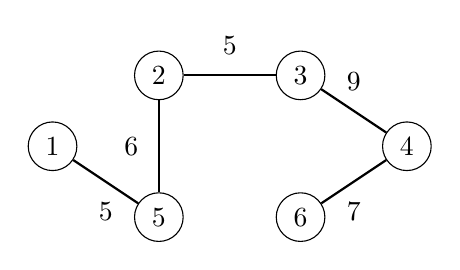
\begin{tikzpicture}[scale=0.9]
\node[draw, circle] (1) at (1.5,2) {$1$};
\node[draw, circle] (2) at (3,3) {$2$};
\node[draw, circle] (3) at (5,3) {$3$};
\node[draw, circle] (4) at (6.5,2) {$4$};
\node[draw, circle] (5) at (3,1) {$5$};
\node[draw, circle] (6) at (5,1) {$6$};
%\path[draw,thick,-] (1) -- node[font=\small,label=above:3] {} (2);
\path[draw,thick,-] (2) -- node[font=\small,label=above:5] {} (3);
\path[draw,thick,-] (3) -- node[font=\small,label=above:9] {} (4);
\path[draw,thick,-] (1) -- node[font=\small,label=below:5] {} (5);
%\path[draw,thick,-] (5) -- node[font=\small,label=below:2] {} (6);
\path[draw,thick,-] (6) -- node[font=\small,label=below:7] {} (4);
\path[draw,thick,-] (2) -- node[font=\small,label=left:6] {} (5);
%\path[draw,thick,-] (3) -- node[font=\small,label=left:3] {} (6);
\end{tikzpicture}
\end{center}

Huomaa, että voi olla monta erilaista
tapaa muodostaa pienin tai
suurin virittävä puu, eli puut eivät ole yksikäsitteisiä.

Tässä luvussa tutustumme algoritmeihin,
jotka muodostavat verkon pienimmän tai suurimman
virittävän puun.
Osoittautuu, että virittävien puiden etsiminen
on siinä mielessä helppo ongelma,
että monenlaiset ahneet menetelmät tuottavat
optimaalisen ratkaisun.

Käymme läpi kaksi algoritmia, jotka molemmat valitsevat
puuhun mukaan kaaria painojärjestyksessä.
Keskitymme pienimmän virittävän puun etsimiseen,
mutta samoilla algoritmeilla voi muodostaa myös suurimman virittävän
puun käsittelemällä kaaret käänteisessä järjestyksessä.

\section{Kruskalin algoritmi}

\index{Kruskalin algoritmi@Kruskalin algoritmi}

\key{Kruskalin algoritmi} aloittaa pienimmän
virittävän
puun muodostamisen tilanteesta,
jossa puussa ei ole yhtään kaaria.
Sitten algoritmi alkaa lisätä
puuhun kaaria järjestyksessä
kevyimmästä raskaimpaan.
Algoritmi lisää kaaren mukaan puuhun,
jos sen lisääminen ei muodosta sykliä.

Kruskalin algoritmi pitää yllä
tietoa verkon komponenteista.
Aluksi jokainen solmu on omassa
komponentissaan,
ja komponentit yhdistyvät pikkuhiljaa
algoritmin aikana puuhun tulevista kaarista.
Lopulta kaikki solmut ovat samassa
komponentissa, jolloin pienin virittävä puu on valmis.

\subsubsection{Esimerkki}

\begin{samepage}
Tarkastellaan Kruskalin algoritmin toimintaa
seuraavassa verkossa:
\begin{center}
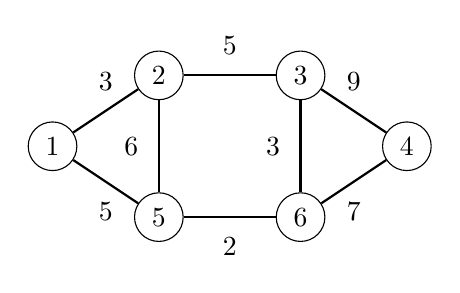
\begin{tikzpicture}[scale=0.9]
\node[draw, circle] (1) at (1.5,2) {$1$};
\node[draw, circle] (2) at (3,3) {$2$};
\node[draw, circle] (3) at (5,3) {$3$};
\node[draw, circle] (4) at (6.5,2) {$4$};
\node[draw, circle] (5) at (3,1) {$5$};
\node[draw, circle] (6) at (5,1) {$6$};
\path[draw,thick,-] (1) -- node[font=\small,label=above:3] {} (2);
\path[draw,thick,-] (2) -- node[font=\small,label=above:5] {} (3);
\path[draw,thick,-] (3) -- node[font=\small,label=above:9] {} (4);
\path[draw,thick,-] (1) -- node[font=\small,label=below:5] {} (5);
\path[draw,thick,-] (5) -- node[font=\small,label=below:2] {} (6);
\path[draw,thick,-] (6) -- node[font=\small,label=below:7] {} (4);
\path[draw,thick,-] (2) -- node[font=\small,label=left:6] {} (5);
\path[draw,thick,-] (3) -- node[font=\small,label=left:3] {} (6);
\end{tikzpicture}
\end{center}
\end{samepage}

\begin{samepage}
Algoritmin ensimmäinen vaihe on
järjestää verkon kaaret niiden painon mukaan.
Tuloksena on seuraava lista:

\begin{tabular}{ll}
\\
kaari & paino \\
\hline
5--6 & 2 \\
1--2 & 3 \\
3--6 & 3 \\
1--5 & 5 \\
2--3 & 5 \\
2--5 & 6 \\
4--6 & 7 \\
3--4 & 9 \\
\\
\end{tabular}
\end{samepage}

Tämän jälkeen algoritmi käy listan läpi
ja lisää kaaren puuhun,
jos se yhdistää kaksi erillistä komponenttia.

Aluksi jokainen solmu on omassa komponentissaan:

\begin{center}
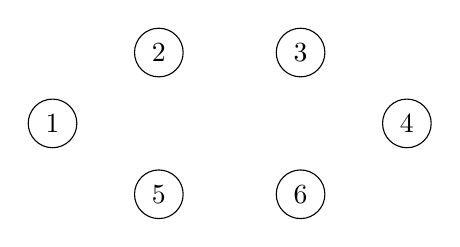
\begin{tikzpicture}[scale=0.9]
\node[draw, circle] (1) at (1.5,2) {$1$};
\node[draw, circle] (2) at (3,3) {$2$};
\node[draw, circle] (3) at (5,3) {$3$};
\node[draw, circle] (4) at (6.5,2) {$4$};
\node[draw, circle] (5) at (3,1) {$5$};
\node[draw, circle] (6) at (5,1) {$6$};
%\path[draw,thick,-] (1) -- node[font=\small,label=above:3] {} (2);
%\path[draw,thick,-] (2) -- node[font=\small,label=above:5] {} (3);
%\path[draw,thick,-] (3) -- node[font=\small,label=above:9] {} (4);
%\path[draw,thick,-] (1) -- node[font=\small,label=below:5] {} (5);
%\path[draw,thick,-] (5) -- node[font=\small,label=below:2] {} (6);
%\path[draw,thick,-] (6) -- node[font=\small,label=below:7] {} (4);
%\path[draw,thick,-] (2) -- node[font=\small,label=left:6] {} (5);
%\path[draw,thick,-] (3) -- node[font=\small,label=left:3] {} (6);
\end{tikzpicture}
\end{center}
Ensimmäinen virittävään puuhun lisättävä
kaari on 5--6, joka yhdistää
komponentit $\{5\}$ ja $\{6\}$ komponentiksi $\{5,6\}$:

\begin{center}
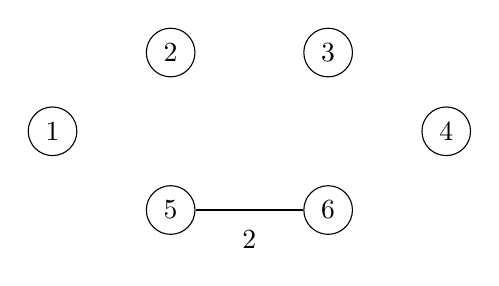
\begin{tikzpicture}
\node[draw, circle] (1) at (1.5,2) {$1$};
\node[draw, circle] (2) at (3,3) {$2$};
\node[draw, circle] (3) at (5,3) {$3$};
\node[draw, circle] (4) at (6.5,2) {$4$};
\node[draw, circle] (5) at (3,1) {$5$};
\node[draw, circle] (6) at (5,1) {$6$};

%\path[draw,thick,-] (1) -- node[font=\small,label=above:3] {} (2);
%\path[draw,thick,-] (2) -- node[font=\small,label=above:5] {} (3);
%\path[draw,thick,-] (3) -- node[font=\small,label=above:9] {} (4);
%\path[draw,thick,-] (1) -- node[font=\small,label=below:5] {} (5);
\path[draw,thick,-] (5) -- node[font=\small,label=below:2] {} (6);
%\path[draw,thick,-] (6) -- node[font=\small,label=below:7] {} (4);
%\path[draw,thick,-] (2) -- node[font=\small,label=left:6] {} (5);
%\path[draw,thick,-] (3) -- node[font=\small,label=left:3] {} (6);
\end{tikzpicture}
\end{center}
Tämän jälkeen algoritmi lisää puuhun vastaavasti
kaaret 1--2, 3--6 ja 1--5:

\begin{center}
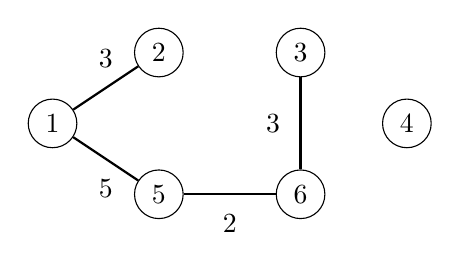
\begin{tikzpicture}[scale=0.9]
\node[draw, circle] (1) at (1.5,2) {$1$};
\node[draw, circle] (2) at (3,3) {$2$};
\node[draw, circle] (3) at (5,3) {$3$};
\node[draw, circle] (4) at (6.5,2) {$4$};
\node[draw, circle] (5) at (3,1) {$5$};
\node[draw, circle] (6) at (5,1) {$6$};

\path[draw,thick,-] (1) -- node[font=\small,label=above:3] {} (2);
%\path[draw,thick,-] (2) -- node[font=\small,label=above:5] {} (3);
%\path[draw,thick,-] (3) -- node[font=\small,label=above:9] {} (4);
\path[draw,thick,-] (1) -- node[font=\small,label=below:5] {} (5);
\path[draw,thick,-] (5) -- node[font=\small,label=below:2] {} (6);
%\path[draw,thick,-] (6) -- node[font=\small,label=below:7] {} (4);
%\path[draw,thick,-] (2) -- node[font=\small,label=left:6] {} (5);
\path[draw,thick,-] (3) -- node[font=\small,label=left:3] {} (6);
\end{tikzpicture}
\end{center}

Näiden lisäysten jälkeen monet
komponentit ovat yhdistyneet ja verkossa on kaksi
komponenttia: $\{1,2,3,5,6\}$ ja $\{4\}$.

Seuraavaksi käsiteltävä kaari on 2--3,
mutta tämä kaari ei tule mukaan puuhun,
koska solmut 2 ja 3 ovat jo samassa komponentissa.
Vastaavasta syystä myöskään kaari 2--5 ei tule mukaan puuhun.

\begin{samepage}
Lopuksi puuhun tulee kaari 4--6,
joka luo yhden komponentin:

\begin{center}
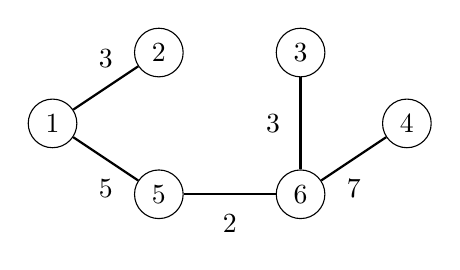
\begin{tikzpicture}[scale=0.9]
\node[draw, circle] (1) at (1.5,2) {$1$};
\node[draw, circle] (2) at (3,3) {$2$};
\node[draw, circle] (3) at (5,3) {$3$};
\node[draw, circle] (4) at (6.5,2) {$4$};
\node[draw, circle] (5) at (3,1) {$5$};
\node[draw, circle] (6) at (5,1) {$6$};

\path[draw,thick,-] (1) -- node[font=\small,label=above:3] {} (2);
%\path[draw,thick,-] (2) -- node[font=\small,label=above:5] {} (3);
%\path[draw,thick,-] (3) -- node[font=\small,label=above:9] {} (4);
\path[draw,thick,-] (1) -- node[font=\small,label=below:5] {} (5);
\path[draw,thick,-] (5) -- node[font=\small,label=below:2] {} (6);
\path[draw,thick,-] (6) -- node[font=\small,label=below:7] {} (4);
%\path[draw,thick,-] (2) -- node[font=\small,label=left:6] {} (5);
\path[draw,thick,-] (3) -- node[font=\small,label=left:3] {} (6);
\end{tikzpicture}
\end{center}
\end{samepage}

Tämän lisäyksen jälkeen algoritmi päättyy,
koska kaikki solmut on kytketty toisiinsa kaarilla
ja verkko on yhtenäinen.
Tuloksena on verkon pienin virittävä puu,
jonka paino on $2+3+3+5+7=20$.

\subsubsection{Miksi algoritmi toimii?}

On hyvä kysymys, miksi Kruskalin algoritmi
toimii aina eli miksi ahne strategia tuottaa
varmasti pienimmän mahdollisen virittävän puun.

Voimme perustella algoritmin toimivuuden
tekemällä vastaoletuksen, että pienimmässä
virittävässä puussa ei olisi verkon keveintä kaarta.
Oletetaan esimerkiksi, että äskeisen verkon
pienimmässä virittävässä puussa ei olisi
2:n painoista kaarta solmujen 5 ja 6 välillä.
Emme tiedä tarkalleen, millainen uusi pienin
virittävä puu olisi, mutta siinä täytyy olla
kuitenkin joukko kaaria.
Oletetaan, että virittävä puu olisi
vaikkapa seuraavanlainen:

\begin{center}
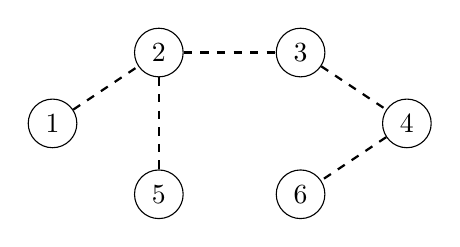
\begin{tikzpicture}[scale=0.9]
\node[draw, circle] (1) at (1.5,2) {$1$};
\node[draw, circle] (2) at (3,3) {$2$};
\node[draw, circle] (3) at (5,3) {$3$};
\node[draw, circle] (4) at (6.5,2) {$4$};
\node[draw, circle] (5) at (3,1) {$5$};
\node[draw, circle] (6) at (5,1) {$6$};

\path[draw,thick,-,dashed] (1) -- (2);
\path[draw,thick,-,dashed] (2) -- (5);
\path[draw,thick,-,dashed] (2) -- (3);
\path[draw,thick,-,dashed] (3) -- (4);
\path[draw,thick,-,dashed] (4) -- (6);
\end{tikzpicture}
\end{center}

Ei ole kuitenkaan mahdollista,
että yllä oleva virittävä puu olisi todellisuudessa
verkon pienin virittävä puu.
Tämä johtuu siitä, että voimme poistaa siitä
jonkin kaaren ja korvata sen 2:n painoisella kaarella.
Tuloksena on virittävä puu, jonka paino on \emph{pienempi}:

\begin{center}
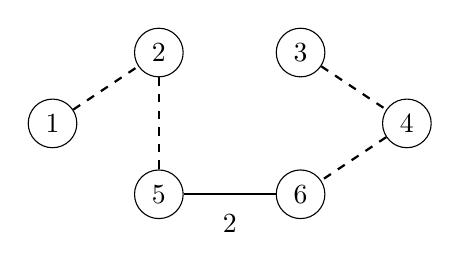
\begin{tikzpicture}[scale=0.9]
\node[draw, circle] (1) at (1.5,2) {$1$};
\node[draw, circle] (2) at (3,3) {$2$};
\node[draw, circle] (3) at (5,3) {$3$};
\node[draw, circle] (4) at (6.5,2) {$4$};
\node[draw, circle] (5) at (3,1) {$5$};
\node[draw, circle] (6) at (5,1) {$6$};

\path[draw,thick,-,dashed] (1) -- (2);
\path[draw,thick,-,dashed] (2) -- (5);
\path[draw,thick,-,dashed] (3) -- (4);
\path[draw,thick,-,dashed] (4) -- (6);
\path[draw,thick,-] (5) -- node[font=\small,label=below:2] {} (6);
\end{tikzpicture}
\end{center}

Niinpä on aina optimaalinen ratkaisu valita pienimpään
virittävään puuhun verkon kevein kaari.
Vastaavalla tavalla on mahdollista perustella
seuraavaksi keveimmän kaaren valinta jne.
Niinpä Kruskalin algoritmi toimii oikein ja
tuottaa aina pienimmän virittävän puun.

\subsubsection{Toteutus}

Kruskalin algoritmi on mukavinta toteuttaa
kaarilistan avulla. Algoritmin ensimmäinen vaihe
on järjestää kaaret painojärjestykseen,
missä kuluu aikaa $O(m \log m)$.
Tämän jälkeen seuraa algoritmin toinen vaihe,
jossa listalta valitaan kaaret mukaan puuhun.

Algoritmin toinen vaihe rakentuu seuraavanlaisen silmukan ympärille:

\begin{lstlisting}
for (...) {
  if (!sama(a,b)) liita(a,b);
}
\end{lstlisting}

Silmukka käy läpi kaikki listan kaaret
niin, että muuttujat $a$ ja $b$ ovat kulloinkin kaaren
päissä olevat solmut.
Koodi käyttää kahta funktiota:
funktio \texttt{sama} tutkii,
ovatko solmut samassa komponentissa,
ja funktio \texttt{liita}
yhdistää kaksi komponenttia toisiinsa.

Ongelmana on, kuinka toteuttaa tehokkaasti
funktiot \texttt{sama} ja \texttt{liita}.
Yksi mahdollisuus on pitää yllä verkkoa tavallisesti
ja toteuttaa funktio \texttt{sama} verkon läpikäyntinä.
Tällöin kuitenkin funktion \texttt{sama}
suoritus veisi aikaa $O(n+m)$,
mikä on hidasta, koska funktiota kutsutaan
jokaisen kaaren kohdalla.

Seuraavaksi esiteltävä union-find-rakenne
ratkaisee asian.
Se toteuttaa molemmat funktiot
ajassa $O(\log n)$,
jolloin Kruskalin algoritmin
aikavaativuus on vain $O(m \log n)$
kaarilistan järjestämisen jälkeen.

\section{Union-find-rakenne}

\index{union-find-rakenne}

\key{Union-find-rakenne} pitää yllä
alkiojoukkoja.
Joukot ovat erillisiä,
eli tietty alkio on tarkalleen
yhdessä joukossa.
Rakenne tarjoaa kaksi operaatiota,
jotka toimivat ajassa $O(\log n)$.
Ensimmäinen operaatio tarkistaa,
ovatko kaksi alkiota samassa joukossa.
Toinen operaatio yhdistää kaksi
joukkoa toisiinsa.

\subsubsection{Rakenne}

Union-find-rakenteessa jokaisella
joukolla on edustaja-alkio.
Kaikki muut joukon alkiot osoittavat
edustajaan joko suoraan tai
muiden alkioiden kautta.

Esimerkiksi jos joukot ovat
$\{1,4,7\}$, $\{5\}$ ja $\{2,3,6,8\}$,
tilanne voisi olla:
\begin{center}
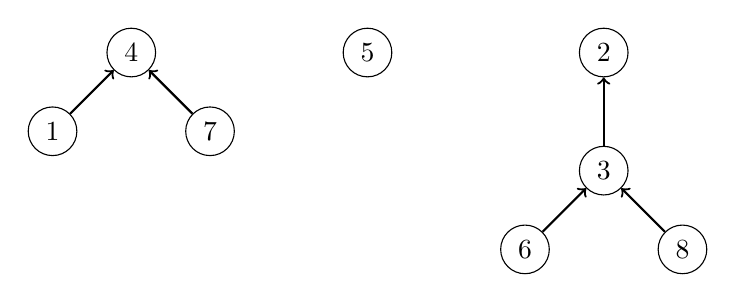
\begin{tikzpicture}
\node[draw, circle] (1) at (0,-1) {$1$};
\node[draw, circle] (2) at (7,0) {$2$};
\node[draw, circle] (3) at (7,-1.5) {$3$};
\node[draw, circle] (4) at (1,0) {$4$};
\node[draw, circle] (5) at (4,0) {$5$};
\node[draw, circle] (6) at (6,-2.5) {$6$};
\node[draw, circle] (7) at (2,-1) {$7$};
\node[draw, circle] (8) at (8,-2.5) {$8$};

\path[draw,thick,->] (1) -- (4);
\path[draw,thick,->] (7) -- (4);

\path[draw,thick,->] (3) -- (2);
\path[draw,thick,->] (6) -- (3);
\path[draw,thick,->] (8) -- (3);

\end{tikzpicture}
\end{center}
Tässä tapauksessa alkiot 4, 5 ja 2
ovat joukkojen edustajat.

Minkä tahansa alkion edustaja
löytyy kulkemalla polku loppuun alkiosta.
Esimerkiksi alkion 6 edustaja on 2,
koska polku on $6 \rightarrow 3 \rightarrow 2$.
Tämän avulla voi selvittää,
ovatko kaksi alkiota samassa joukossa:
jos kummankin alkion edustaja on sama,
alkiot ovat samassa joukossa,
ja muuten eri joukoissa.

Joukkojen yhdistäminen tapahtuu
valitsemalla toisen edustaja
joukkojen yhteiseksi edustajaksi
ja kytkemällä toinen edustaja siihen.
Esimerkiksi joukot $\{1,4,7\}$ ja $\{2,3,6,8\}$
voi yhdistää näin joukoksi $\{1,2,3,4,6,7,8\}$:
\begin{center}
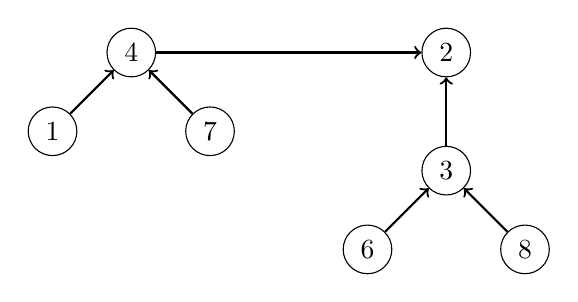
\begin{tikzpicture}
\node[draw, circle] (1) at (2,-1) {$1$};
\node[draw, circle] (2) at (7,0) {$2$};
\node[draw, circle] (3) at (7,-1.5) {$3$};
\node[draw, circle] (4) at (3,0) {$4$};
\node[draw, circle] (6) at (6,-2.5) {$6$};
\node[draw, circle] (7) at (4,-1) {$7$};
\node[draw, circle] (8) at (8,-2.5) {$8$};

\path[draw,thick,->] (1) -- (4);
\path[draw,thick,->] (7) -- (4);

\path[draw,thick,->] (3) -- (2);
\path[draw,thick,->] (6) -- (3);
\path[draw,thick,->] (8) -- (3);

\path[draw,thick,->] (4) -- (2);
\end{tikzpicture}
\end{center}

Joukkojen yhteiseksi edustajaksi valitaan alkio 2,
minkä vuoksi alkio 4 yhdistetään siihen.
Tästä lähtien alkio 2 edustaa kaikkia joukon alkioita.

Tehokkuuden kannalta oleellista on,
miten yhdistäminen tapahtuu.
Osoittautuu, että ratkaisu on yksinkertainen:
riittää yhdistää aina pienempi joukko suurempaan,
tai kummin päin tahansa,
jos joukot ovat yhtä suuret.
Tällöin pisin ketju
alkiosta edustajaan on aina luokkaa $O(\log n)$,
koska jokainen askel eteenpäin
ketjussa kaksinkertaistaa
vastaavan joukon koon.

\subsubsection{Toteutus}

Union-find-rakenne on kätevää toteuttaa
taulukoiden avulla.
Seuraavassa toteutuksessa taulukko \texttt{k}
viittaa seuraavaan alkioon ketjussa
tai alkioon itseensä, jos alkio on edustaja.
Taulukko \texttt{s} taas kertoo jokaiselle edustajalle,
kuinka monta alkiota niiden joukossa on.

Aluksi jokainen alkio on omassa joukossaan,
jonka koko on 1:

\begin{lstlisting}
for (int i = 1; i <= n; i++) k[i] = i;
for (int i = 1; i <= n; i++) s[i] = 1;
\end{lstlisting}

Funktio \texttt{id} kertoo alkion $x$
joukon edustajan. Alkion edustaja löytyy
käymällä ketju läpi alkiosta $x$ alkaen.

\begin{lstlisting}
int id(int x) {
    while (x != k[x]) x = k[x];
    return x;
}
\end{lstlisting}

Funktio \texttt{sama} kertoo,
ovatko alkiot $a$ ja $b$ samassa joukossa.
Tämä onnistuu helposti funktion
\texttt{id} avulla.

\begin{lstlisting}
bool sama(int a, int b) {
    return id(a) == id(b);
}
\end{lstlisting}

\begin{samepage}
Funktio \texttt{liita} yhdistää
puolestaan alkioiden $a$ ja $b$ osoittamat
joukot yhdeksi joukoksi.
Funktio etsii ensin joukkojen edustajat
ja yhdistää sitten pienemmän joukon suurempaan.

\begin{lstlisting}
void liita(int a, int b) {
    a = id(a);
    b = id(b);
    if (s[b] > s[a]) swap(a,b);
    s[a] += s[b];
    k[b] = a;
}
\end{lstlisting}
\end{samepage}

Funktion \texttt{id} aikavaativuus on $O(\log n)$
olettaen, että ketjun pituus on luokkaa $O(\log n)$.
Niinpä myös funktioiden \texttt{sama} ja \texttt{liita}
aikavaativuus on $O(\log n)$.
Funktio \texttt{liita} varmistaa,
että ketjun pituus on luokkaa $O(\log n)$
yhdistämällä pienemmän joukon suurempaan.

% Funktiota \texttt{id} on mahdollista vielä tehostaa
% seuraavasti:
% 
% \begin{lstlisting}
% int id(int x) {
%   if (x == k[x]) return x;
%   return k[x] = id(x);
% }
% \end{lstlisting}
% 
% Nyt joukon edustajan etsimisen yhteydessä kaikki ketjun
% alkiot laitetaan osoittamaan suoraan edustajaan.
% On mahdollista osoittaa, että tämän avulla
% funktioiden \texttt{sama} ja \texttt{liita}
% aikavaativuus on tasoitetusti
% vain $O(\alpha(n))$, missä $\alpha(n)$ on
% hyvin hitaasti kasvava käänteinen Ackermannin funktio.

\section{Primin algoritmi}

\index{Primin algoritmi@Primin algoritmi}

\key{Primin algoritmi} on vaihtoehtoinen menetelmä
verkon pienimmän virittävän puun muodostamiseen.
Algoritmi aloittaa puun muodostamisen valitusta
verkon solmusta ja lisää puuhun aina kaaren,
joka on mahdollisimman kevyt ja joka
liittää puuhun uuden solmun.
Lopulta kaikki solmut on lisätty puuhun
ja pienin virittävä puu on valmis.

Primin algoritmin toiminta on lähellä
Dijkstran algoritmia.
Erona on, että Dijkstran algoritmissa valitaan
kaari, jonka kautta syntyy lyhin polku alkusolmusta
uuteen solmuun, mutta Primin algoritmissa
valitaan vain kevein kaari, joka johtaa uuteen solmuun.

\subsubsection{Esimerkki}

Tarkastellaan Primin algoritmin toimintaa
seuraavassa verkossa:

\begin{center}
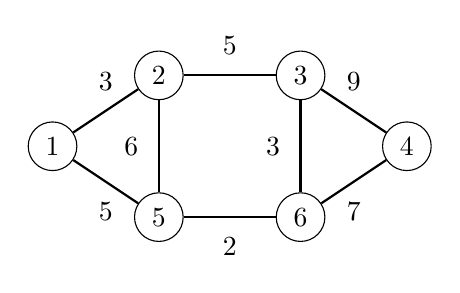
\begin{tikzpicture}[scale=0.9]
\node[draw, circle] (1) at (1.5,2) {$1$};
\node[draw, circle] (2) at (3,3) {$2$};
\node[draw, circle] (3) at (5,3) {$3$};
\node[draw, circle] (4) at (6.5,2) {$4$};
\node[draw, circle] (5) at (3,1) {$5$};
\node[draw, circle] (6) at (5,1) {$6$};
\path[draw,thick,-] (1) -- node[font=\small,label=above:3] {} (2);
\path[draw,thick,-] (2) -- node[font=\small,label=above:5] {} (3);
\path[draw,thick,-] (3) -- node[font=\small,label=above:9] {} (4);
\path[draw,thick,-] (1) -- node[font=\small,label=below:5] {} (5);
\path[draw,thick,-] (5) -- node[font=\small,label=below:2] {} (6);
\path[draw,thick,-] (6) -- node[font=\small,label=below:7] {} (4);
\path[draw,thick,-] (2) -- node[font=\small,label=left:6] {} (5);
\path[draw,thick,-] (3) -- node[font=\small,label=left:3] {} (6);

%\path[draw=red,thick,-,line width=2pt] (5) -- (6);
\end{tikzpicture}
\end{center}

Aluksi solmujen välillä ei ole mitään kaaria:
\begin{center}
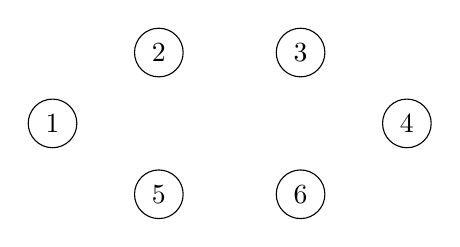
\begin{tikzpicture}[scale=0.9]
\node[draw, circle] (1) at (1.5,2) {$1$};
\node[draw, circle] (2) at (3,3) {$2$};
\node[draw, circle] (3) at (5,3) {$3$};
\node[draw, circle] (4) at (6.5,2) {$4$};
\node[draw, circle] (5) at (3,1) {$5$};
\node[draw, circle] (6) at (5,1) {$6$};
%\path[draw,thick,-] (1) -- node[font=\small,label=above:3] {} (2);
%\path[draw,thick,-] (2) -- node[font=\small,label=above:5] {} (3);
%\path[draw,thick,-] (3) -- node[font=\small,label=above:9] {} (4);
%\path[draw,thick,-] (1) -- node[font=\small,label=below:5] {} (5);
%\path[draw,thick,-] (5) -- node[font=\small,label=below:2] {} (6);
%\path[draw,thick,-] (6) -- node[font=\small,label=below:7] {} (4);
%\path[draw,thick,-] (2) -- node[font=\small,label=left:6] {} (5);
%\path[draw,thick,-] (3) -- node[font=\small,label=left:3] {} (6);
\end{tikzpicture}
\end{center}

Puun muodostuksen voi aloittaa mistä tahansa solmusta,
ja aloitetaan se nyt solmusta 1.
Kevein kaari on painoltaan 3 ja se johtaa solmuun 2:
\begin{center}
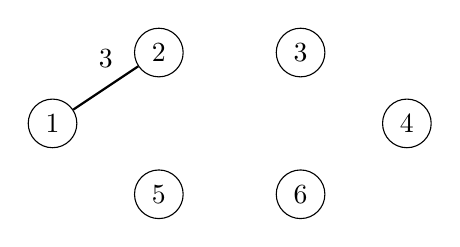
\begin{tikzpicture}[scale=0.9]
\node[draw, circle] (1) at (1.5,2) {$1$};
\node[draw, circle] (2) at (3,3) {$2$};
\node[draw, circle] (3) at (5,3) {$3$};
\node[draw, circle] (4) at (6.5,2) {$4$};
\node[draw, circle] (5) at (3,1) {$5$};
\node[draw, circle] (6) at (5,1) {$6$};
\path[draw,thick,-] (1) -- node[font=\small,label=above:3] {} (2);
%\path[draw,thick,-] (2) -- node[font=\small,label=above:5] {} (3);
%\path[draw,thick,-] (3) -- node[font=\small,label=above:9] {} (4);
%\path[draw,thick,-] (1) -- node[font=\small,label=below:5] {} (5);
%\path[draw,thick,-] (5) -- node[font=\small,label=below:2] {} (6);
%\path[draw,thick,-] (6) -- node[font=\small,label=below:7] {} (4);
%\path[draw,thick,-] (2) -- node[font=\small,label=left:6] {} (5);
%\path[draw,thick,-] (3) -- node[font=\small,label=left:3] {} (6);
\end{tikzpicture}
\end{center}

Nyt kevein uuteen solmuun johtavan
kaaren paino on 5,
ja voimme laajentaa joko solmuun 3 tai 5.
Valitaan solmu 3:
\begin{center}
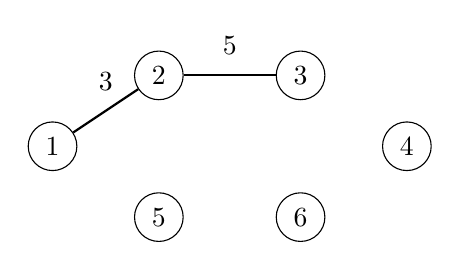
\begin{tikzpicture}[scale=0.9]
\node[draw, circle] (1) at (1.5,2) {$1$};
\node[draw, circle] (2) at (3,3) {$2$};
\node[draw, circle] (3) at (5,3) {$3$};
\node[draw, circle] (4) at (6.5,2) {$4$};
\node[draw, circle] (5) at (3,1) {$5$};
\node[draw, circle] (6) at (5,1) {$6$};
\path[draw,thick,-] (1) -- node[font=\small,label=above:3] {} (2);
\path[draw,thick,-] (2) -- node[font=\small,label=above:5] {} (3);
%\path[draw,thick,-] (3) -- node[font=\small,label=above:9] {} (4);
%\path[draw,thick,-] (1) -- node[font=\small,label=below:5] {} (5);
%\path[draw,thick,-] (5) -- node[font=\small,label=below:2] {} (6);
%\path[draw,thick,-] (6) -- node[font=\small,label=below:7] {} (4);
%\path[draw,thick,-] (2) -- node[font=\small,label=left:6] {} (5);
%\path[draw,thick,-] (3) -- node[font=\small,label=left:3] {} (6);
\end{tikzpicture}
\end{center}

\begin{samepage}
Sama jatkuu, kunnes kaikki solmut ovat mukana puussa:
\begin{center}
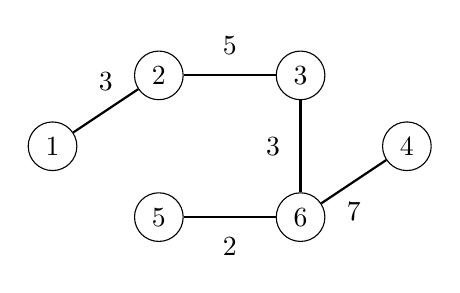
\begin{tikzpicture}[scale=0.9]
\node[draw, circle] (1) at (1.5,2) {$1$};
\node[draw, circle] (2) at (3,3) {$2$};
\node[draw, circle] (3) at (5,3) {$3$};
\node[draw, circle] (4) at (6.5,2) {$4$};
\node[draw, circle] (5) at (3,1) {$5$};
\node[draw, circle] (6) at (5,1) {$6$};
\path[draw,thick,-] (1) -- node[font=\small,label=above:3] {} (2);
\path[draw,thick,-] (2) -- node[font=\small,label=above:5] {} (3);
%\path[draw,thick,-] (3) -- node[font=\small,label=above:9] {} (4);
%\path[draw,thick,-] (1) -- node[font=\small,label=below:5] {} (5);
\path[draw,thick,-] (5) -- node[font=\small,label=below:2] {} (6);
\path[draw,thick,-] (6) -- node[font=\small,label=below:7] {} (4);
%\path[draw,thick,-] (2) -- node[font=\small,label=left:6] {} (5);
\path[draw,thick,-] (3) -- node[font=\small,label=left:3] {} (6);
\end{tikzpicture}
\end{center}
\end{samepage}

\subsubsection{Algoritmin toteutus}

Dijkstran algoritmin tavoin Primin algoritmin voi toteuttaa
tehokkaasti käyttämällä prioriteettijonoa.
Primin algoritmin tapauksessa jono sisältää kaikki solmut,
jotka voi yhdistää nykyiseen komponentiin kaarella,
järjestyksessä kaaren painon mukaan kevyimmästä raskaimpaan.

Primin algoritmin aikavaativuus on $O(n + m \log m)$
eli sama kuin Dijkstran algoritmissa.
Käytännössä Primin algoritmi on suunnilleen
yhtä nopea kuin Kruskalin algoritmi,
ja onkin makuasia, kumpaa algoritmia käyttää.
Useimmat kisakoodarit käyttävät Kruskalin algoritmia.


